\section{Further Numerical Experiments}
% \label{appn:experiments}

\subsection{Run Time for Varying $\varepsilon$}
\begin{figure}
    \centering
    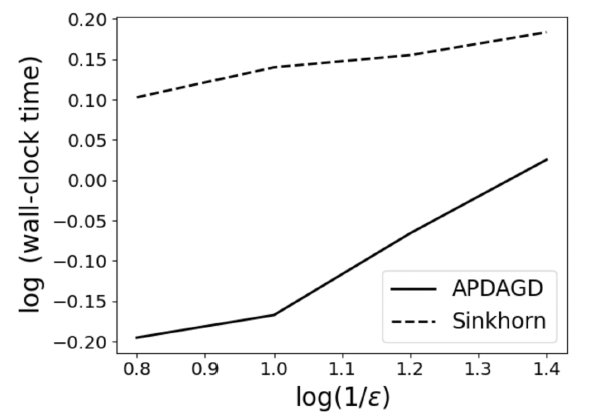
\includegraphics[width=0.5\linewidth]{figs/runtime_vary_eps.png}
    \caption{Comparison of wall-clock running time between APDAGD and Sinkhorn for varying $\varepsilon$}
    \label{fig:runtime_for_varying_epsilon}
\end{figure}
With the similar setting to Figure \ref{fig:de_vs_apdagd} of using images in the CIFAR-10 dataset, we provide additional experiments showcasing that APDAGD is better than Sinkhorn in wall-clock time in terms of both aggregate run time cost in Figure \ref{fig:runtime_for_varying_epsilon}. Moreover, for aggregate wall-clock time, we note that previous works showed that gradient methods and especially APDAGD are practically faster than Sinkhorn \cite[Figure 1]{Dvurechensky-2018-Computational}. This claim is further supported by Figure \ref{fig:runtime_for_varying_epsilon} since it reproduce the results from \cite[Figure 1]{Dvurechensky-2018-Computational} which compare the runtime of Sinkhorn and APDAGD in the context of OT. 
\subsection{Revised Sinkhorn}
We again utilize the same setting Figure \ref{fig:de_vs_apdagd} and Run Time for Varying $\varepsilon$ with CIFAR-10 dataset. On the left, we empirically verify our theoretical bounds in Theorem \ref{contraint_violation}, by showing that increasing $A$ potentially lead to a better feasibility of Sinkhorn. For the figure on the right, we show that the increase of $A$ to a sufficient size can lead to more number of iterations to convergence of Sinkhorn. This is also suggested by the worsened theoretical complexity of revised Sinkhorn (Theorem \ref{them:revised_sinkhorn_complexity}).
\begin{figure}
    \centering
    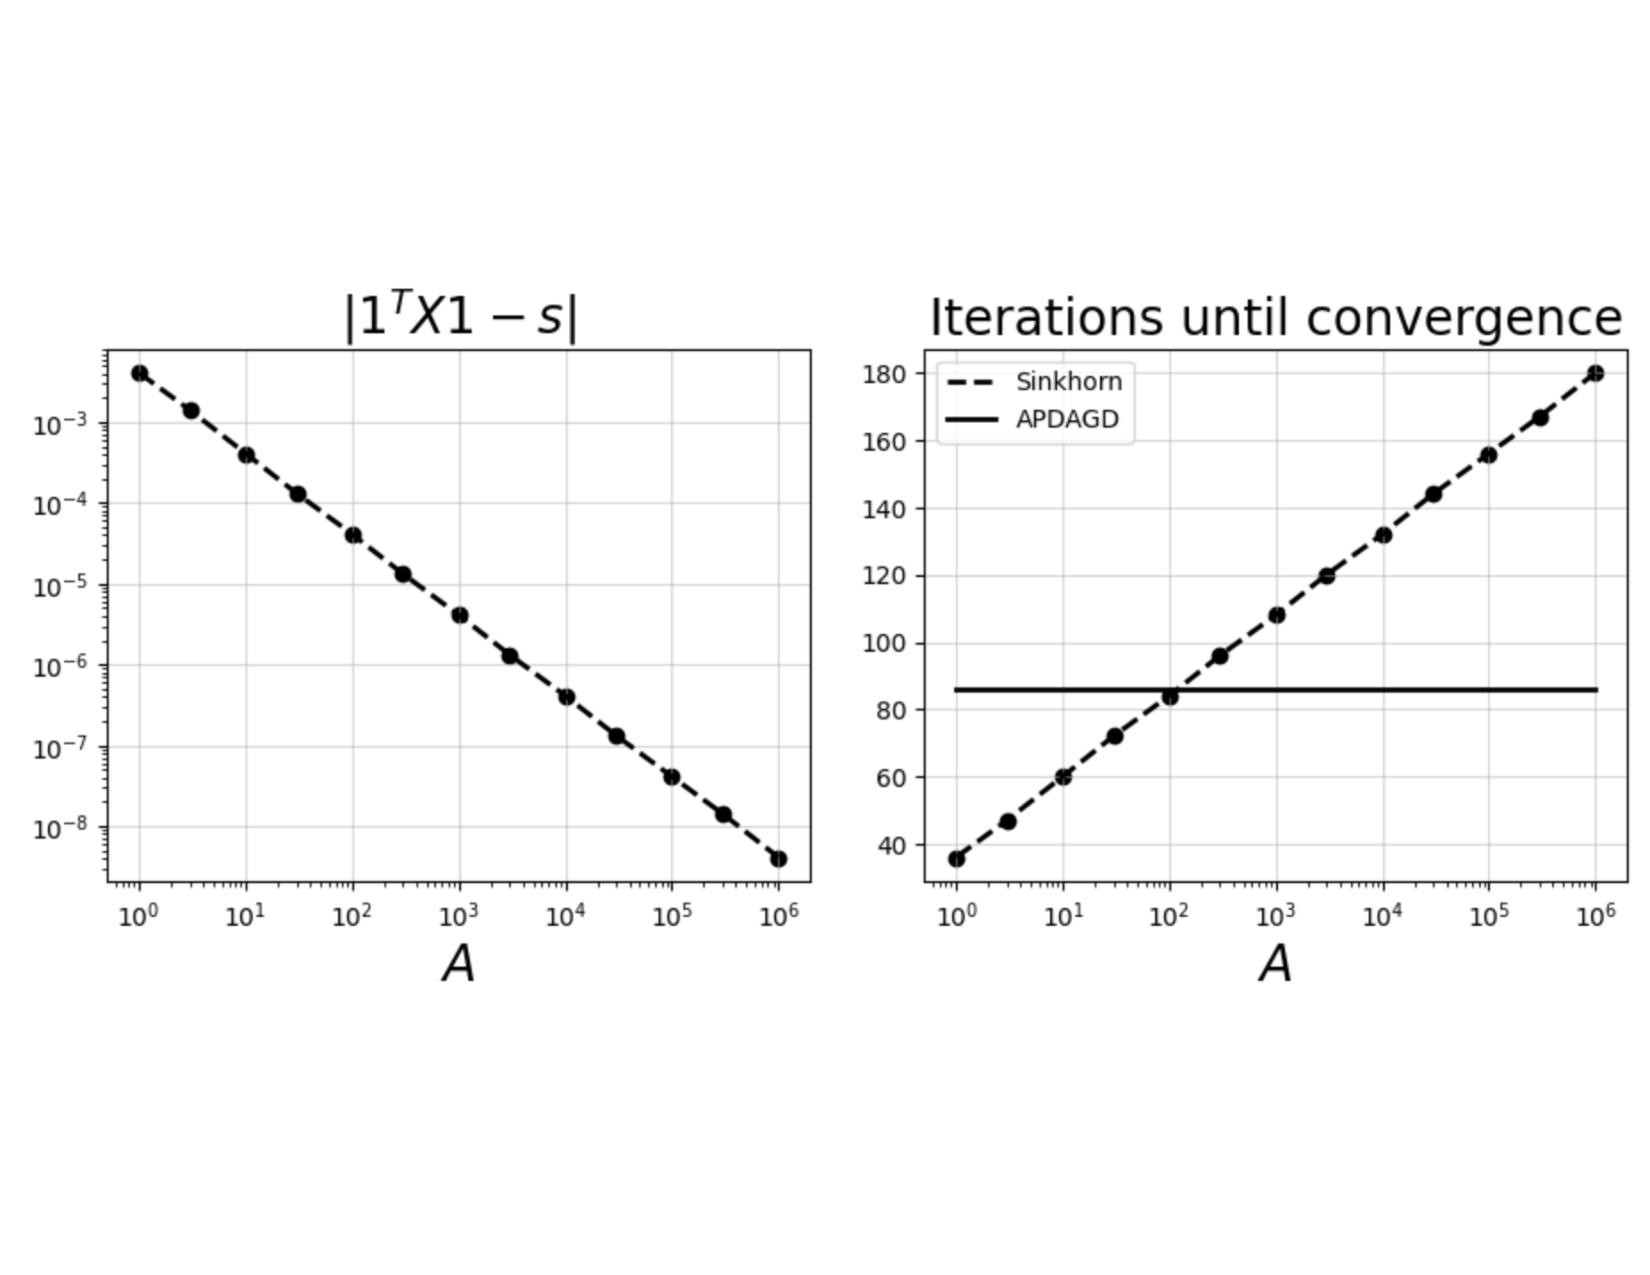
\includegraphics[width=0.8\linewidth]{figs/revised_sinkhorn.pdf}
    \caption{Left: Sinkhorn constraint violation with respect to $A$. Right: Number of iterations for both APDAGD and Sinkhorn until a pre-defined suboptimality is achieved.}
    \label{fig:revised_sinkhorn}
\end{figure}

\subsection{Domain Adaptation}
In our setting, the source and target datasets contain different numbers of data points ($N_s = 300$ and $N_t = 400$, respectively). For OT, we use Sinkhorn to approximate the OT matrix of size 300 $\times$ 400, then transform the source examples according to Courty et al. (2017). For POT, we use K-means clustering to transform the target domains to a histogram of $300$ bins. The two unbalanced marginals are then normalized so that $\left\| r \right\|_1 = 0.75, \left\| c \right\|_1 = 1.0$, and we set $s = 0.999 \times \min\{ \left\| r \right\|_1, \left\| c \right\|_1 \}$ then use APDAGD to find the POT matrix between these two unbalanced marginals. The source examples are transformed similarly. Finally, for both methods (OT and POT), we train a support vector machine with the radial basis kernel (parameter $\sigma^2 = 1$) using the transformed source domain. In the Figure \ref{fig:POT_vs_OT} we report the accuracy on the target domain using 20,000 test examples. All hyperparameters are set to be equal.


Here we implement and compare Domain Adaptation with OT to Domain Adaptation with POT, which is calculated with two different algorithms Sinkhorn (infeasible rounding) and APDAGD (with our novel \textsc{Round-POT}). In \citep{courty2017joint}, the authors presented an OT-based method to transform a source domain to a reference target domain such that the their densities are approximately equal. We present a binary classification setting involving the "moons" dataset. The source dataset is displayed as colored scatter points. The target dataset comes from the same distribution, but the points go to a rotation of 60 degrees (black scatter points), representing a domain covariate shift. Additional experimental details are further described in Further Experiments Setup Details section in Appendix. % We then use APDAGD to find the POT matrix between these two unbalanced marginals. The source examples are transformed similarly. Finally, for both methods (OT and POT), we train a support vector machine with the radial basis kernel (parameter $\sigma^2 = 1$) using the transformed source domain. 
To summarize the results, POT offers much more practicality as it does not require normalizing both marginals to have a sum of 1 in contrast to OT. More importantly, POT avoids bad matchings to outliers due to the flexibility in choosing the amount of mass transported, resulting in a higher accuracy than OT. Furthermore, linking back to Remark \ref{remark:violation}, the infeasibility Sinkhorn degrades the practical performance of POT for Domain Adaption and consequently leads to a worse accuracy compared APDAGD. This is because the optimal mapping between the source and target domains requires the exact fraction of mass to be transported which APDAGD fulfills practically in contrast to Sinkhorn.  

\begin{figure}
    \centering
    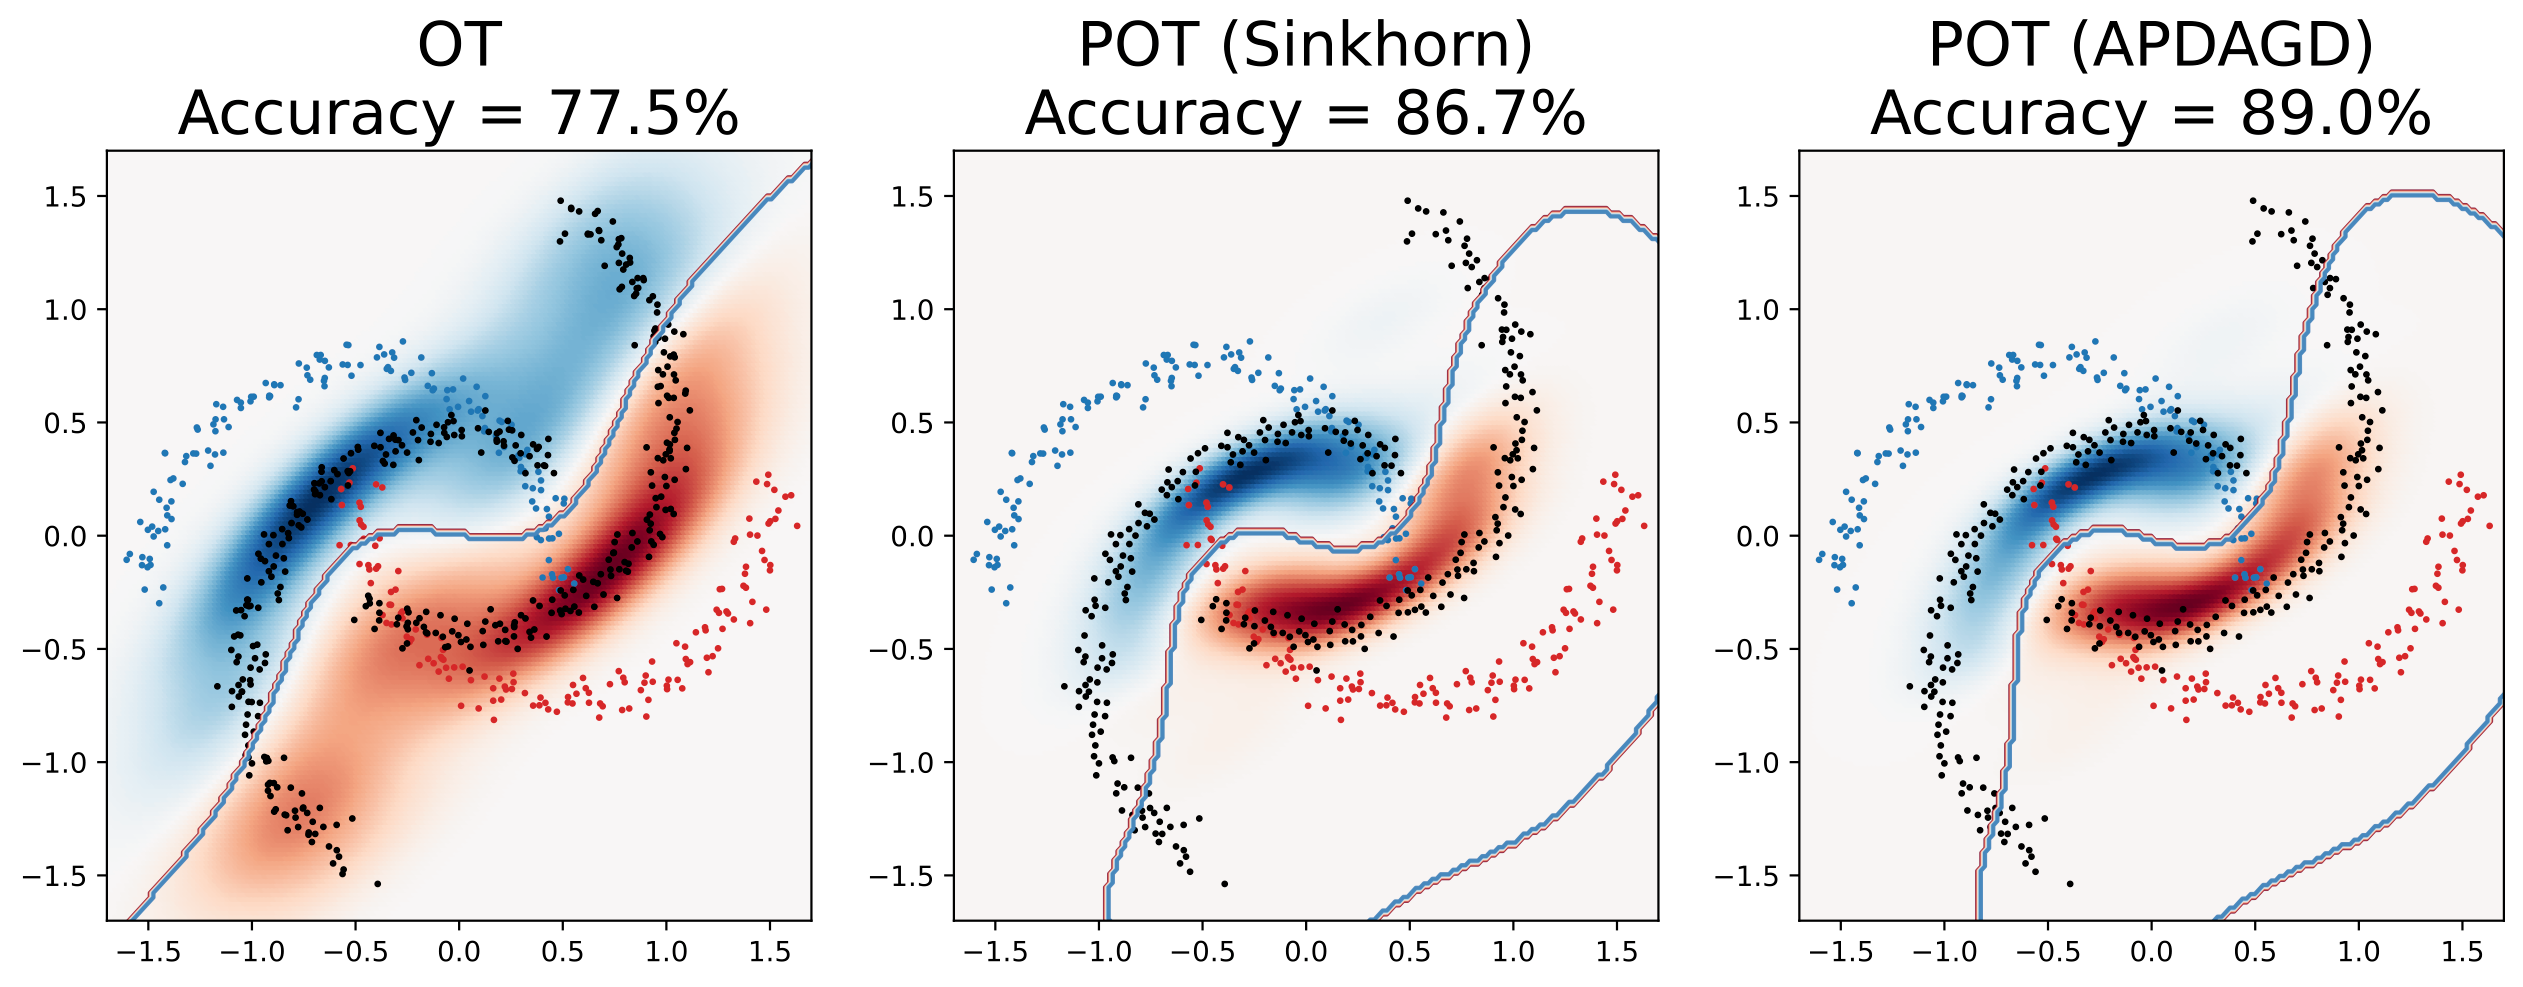
\includegraphics[width=1\linewidth]{figs/POT_vs_OT.png}
    \caption{Domain adaptation with OT and with POT. POT offers a flexibility in choosing the mass transported and helps avoid the need to normalize both marginals to have a sum of $1$, resulting in better complexity than OT. APDAGD demonstrates better accuracy in the novel domain than Sinkhorn, which suffers from infeasibility.}
    \label{fig:POT_vs_OT}
\end{figure}

\subsection{Synthetic Data}
\begin{figure}[ht]
    \centering
    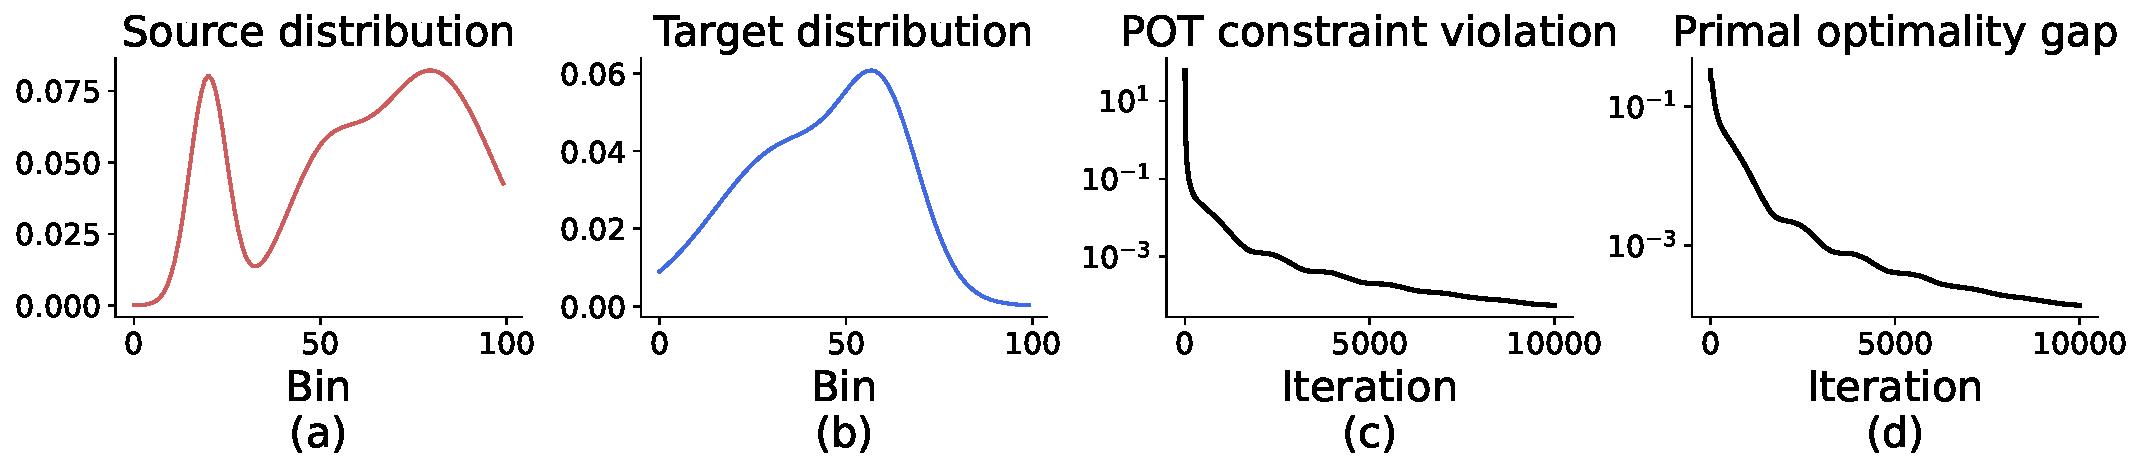
\includegraphics[width=1\linewidth]{figs/apdagd_synthetic.pdf}
    \caption{Convergence of APDAGD on a synthetic setting.}
    \label{fig:apdagd_synthetic}
\end{figure}

In this section we design a POT setting and evaluate the convergence of APDAGD. The two marginals are unnormalized Gaussian mixtures. We then discretize them into histograms of $n = 100$ bins each and perform normalization so that $\norm{\vr}_1 = 5$, $\norm{\vc}_1 = 3$. The total transported mass is set to $s = 0.9 \min\{ \norm{\vr}_1, \norm{\vc}_1 \} = 2.7$, and the cost matrix represents squared Euclidean distances between every pair of bins in the source and target histograms. In other words, $C_{i, j} = (i - j)^2$ for all $i, j = 1, \ldots, n$. Finally, we divide $\vC$ by its maximum entry to have $\norm{\vC}_\text{max} = 1$.

We use \texttt{cvxpy} with the GUROBI backend to solve the linear problem \eqref{prob:pot_with_pq}, and denote by $f^*$ the optimal objective value. This will be used to calculate the primal optimality gap.

The approximate POT solution is solved using APDAGD, where we set the additive suboptimality error $\varepsilon$ to $10^{-3}$. We run APDAGD for 10,000 iterations and keep track of two errors. The first error is constraint violation, equal to $\norm{\vX \ones + \vp - \vr}_1 + \norm{\vX^\top \ones + \vq - \vc}_1 + \lvert \ones^\top \vX \ones - s \rvert$ where $\vX$, $\vp$ and $\vq$ are part of the solution $\vx_k$ found after each iteration. The second error is the optimality gap for the primal objective. To calculate this, we need to round the solution so that it becomes primal feasible. We use our rounding algorithm described in Rounding Algorithm Section to round $\vX$, $\vp$, and $\vq$ after each iteration, giving us $\bar{\vX}$, $\bar{\vp}$ and $\bar{\vq}$. The primal gap then is $\inner{\vC}{\bar{\vX}} - f^*$.

% \subsection{Extra Details for Domain Adaptation}
% Here we provide a new experimental result in domain adaptation. In Courty et al. (2017), the authors presented an OT-based method to transform a source domain to a reference target domain such that the their densities are approximately equal. We present a binary classification setting involving the "moons" dataset. The source dataset is displayed as colored scatter points. The target dataset comes from the same distribution, but the points go to a rotation of 60 degrees (black scatter points below), representing a domain covariate shift.

% In our setting, the source and target datasets contain different numbers of data points ($N_s = 300$ and $N_t = 400$, respectively). For OT, we use Sinkhorn to approximate the OT matrix of size 300 $\times$ 400, then transform the source examples according to Courty et al. (2017). For POT, we use K-means clustering to transform the target domains to a histogram of $300$ bins. The two unbalanced marginals are then normalized so that $\left\| r \right\|_1 = 0.75, \left\| c \right\|_1 = 1.0$, and we set $s = 0.999 \times \min\{ \left\| r \right\|_1, \left\| c \right\|_1 \}$ then use APDAGD to find the POT matrix between these two unbalanced marginals. The source examples are transformed similarly. Finally, for both methods (OT and POT), we train a support vector machine with the radial basis kernel (parameter $\sigma^2 = 1$) using the transformed source domain. In the figure below we report the accuracy on the target domain using 20,000 test examples. POT offers a flexibility in choosing the mass transported and helps avoid the need to normalize both marginals to have a sum of $1$. POT also results in a higher accuracy than OT.

% \begin{figure}
%     \centering
%     \includegraphics[width=1\linewidth]{figs/POT vs OT.png}
%     \caption{Domain Adaptation with OT vs with POT}
%     \label{fig:POT_vs_OT}
% \end{figure}

% In figure \ref{fig:Sinkhorn_vs_APDAGD}, we additionally compare two methods of approximating the POT matrix in this paper: Sinkhorn (which outputs a primal infeasible solution) and APDAGD. All hyperparameters are equal. The results indicate that, in addition to giving a primal feasible solution, APDAGD gives a higher accuracy than Sinkhorn.  
% % \begin{figure}
% %     \centering
% %     \includegraphics[width=1\linewidth]{figs/Sinkhorn vs APDAGD.png}
% %     \caption{Domain Adaptation by APDAGD vs by Sinkhorn}
% %     \label{fig:Sinkhorn_vs_APDAGD}
% % \end{figure}

\subsection{Scalability of APDAGD}
Given the complexity claims in the paper, it is important to show how running time scales with $n$, the number of supports in each marginal. In the below Figure \ref{fig:scalability}, we show the wall-clock time of running APDAGD to solve the POT problem between two Gaussian mixtures (shown in the end of the appendix). We fix the error tolerance to $\varepsilon = 10^{-1}$ and vary $n$ in the set $\{ 10, 30, 100, 300, 1000, 3000, 10000 \}$. The figure plots wall-clock time in seconds against $n$. The expected slope of the best-fit line between $\log(\text{time})$ and $\log(n)$ should be at most 2.5, as the complexity is $\widetilde{O}(n^{2.5} / \varepsilon)$. We find that the slope is $2.19$, which is consistent with the upper bound. Furthermore, the correlation is statistically significant.

\begin{figure}
    \centering
    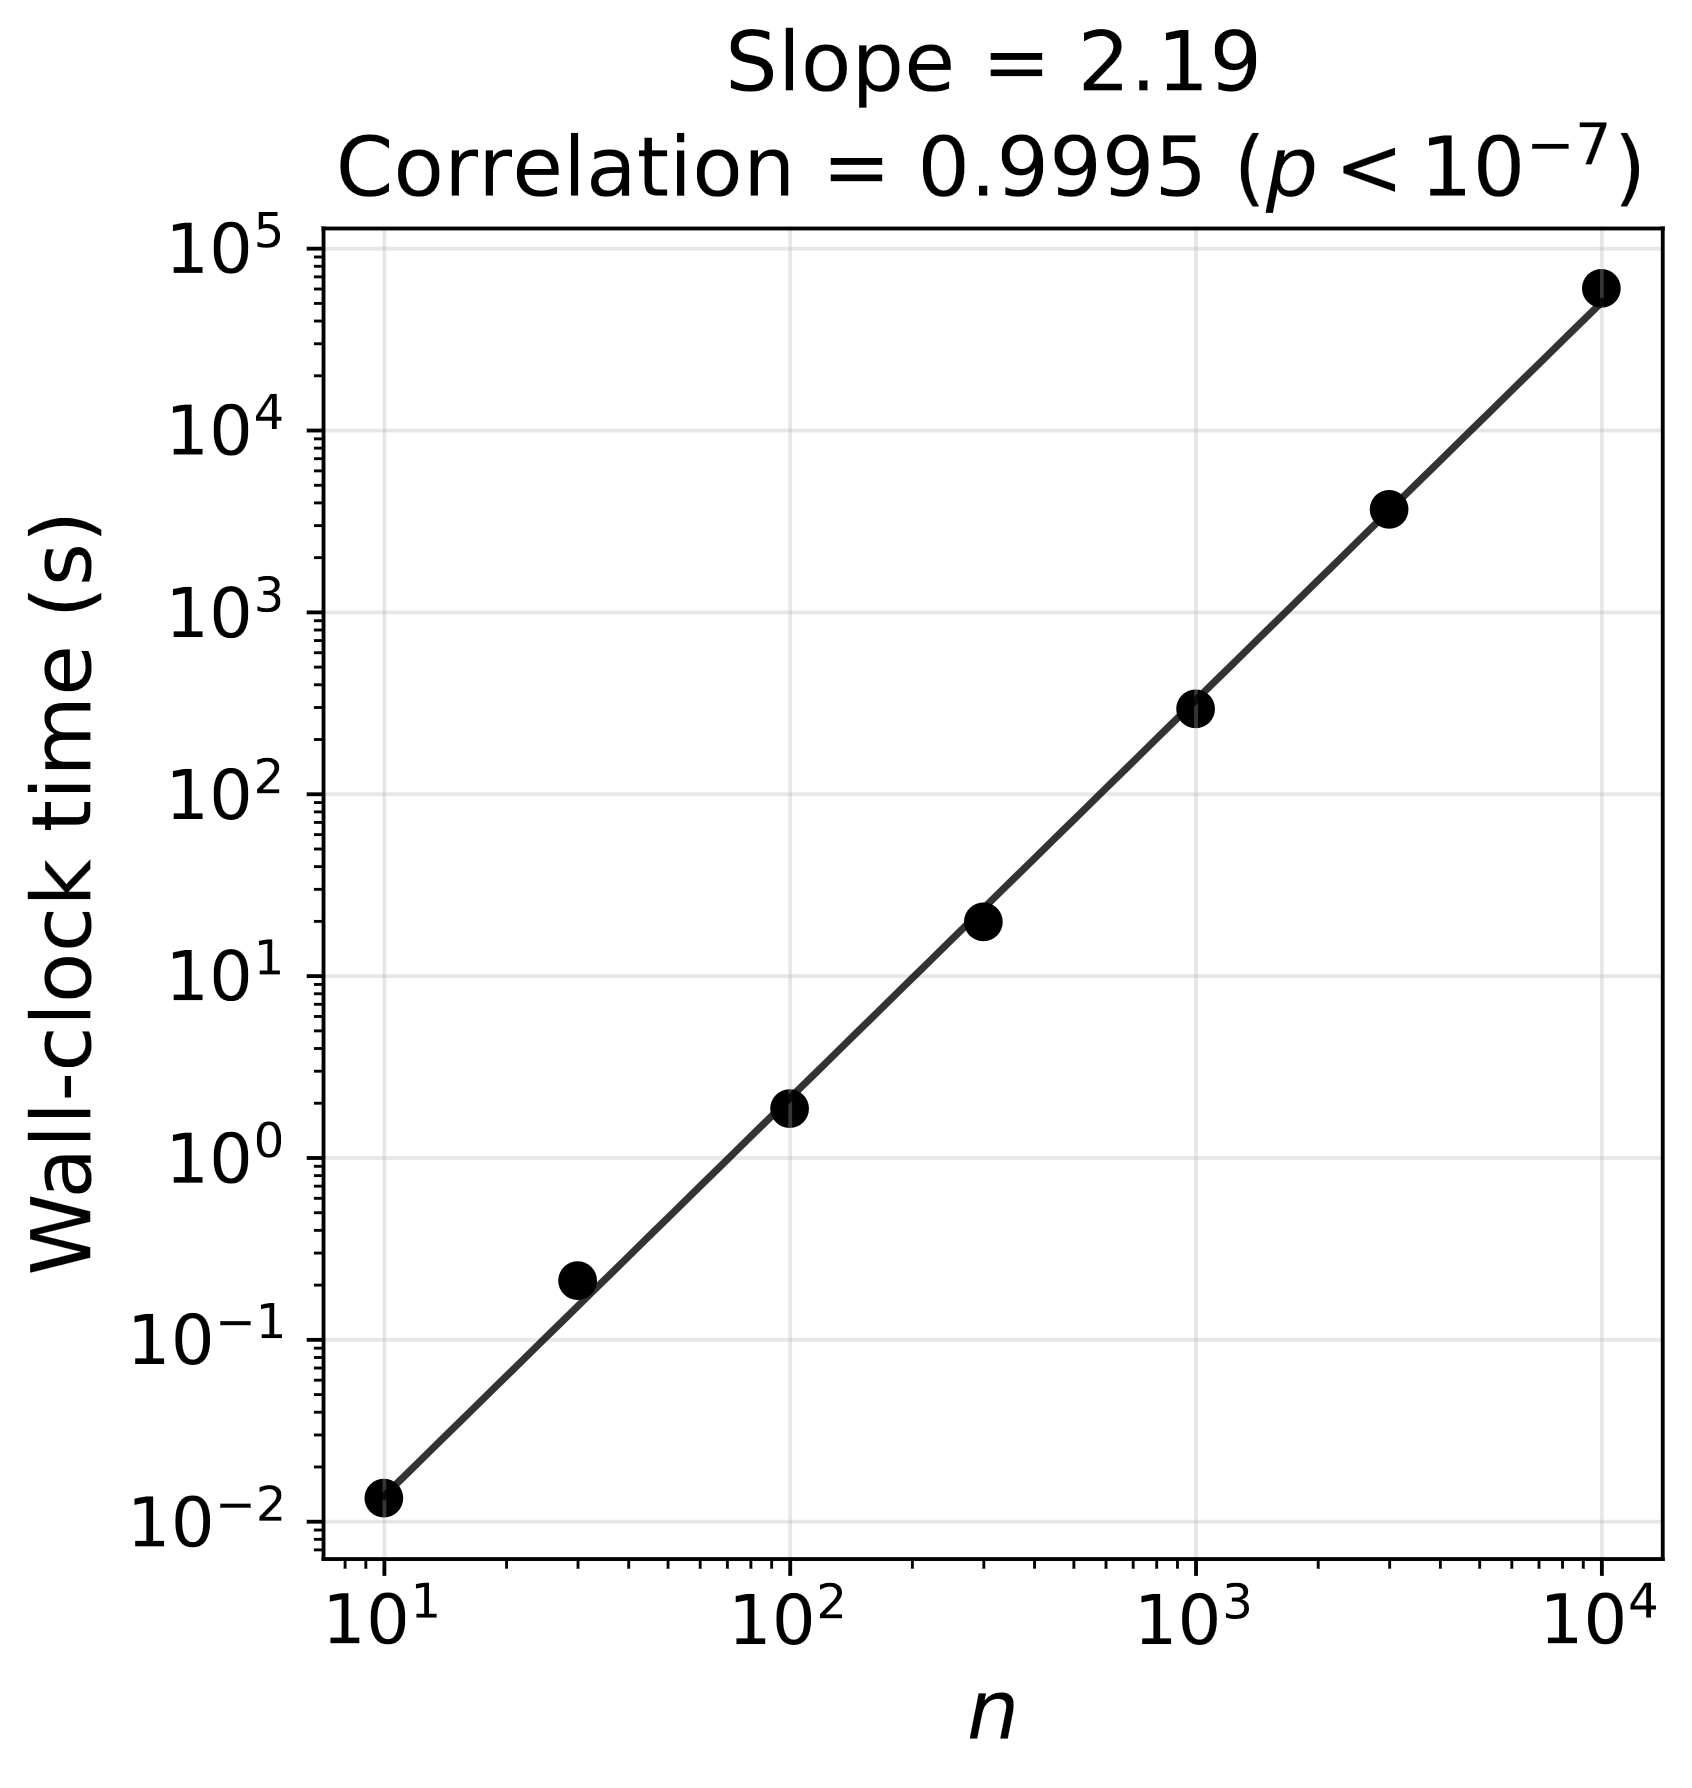
\includegraphics[width=0.4\linewidth]{figs/scalability.png}
    \caption{Wall-clock time of solving POT with APDAGD against $n$}
    \label{fig:scalability}
\end{figure}

\newpage

